% This is samplepaper.tex, a sample chapter demonstrating the
% LLNCS macro package for Springer Computer Science proceedings;
% Version 2.21 of 2022/01/12
%
\documentclass[runningheads]{llncs}
%
\usepackage[T1]{fontenc}
% T1 fonts will be used to generate the final print and online PDFs,
% so please use T1 fonts in your manuscript whenever possible.
% Other font encondings may result in incorrect characters.
%
\usepackage{graphicx}
% Used for displaying a sample figure. If possible, figure files should
% be included in EPS format.
%
% If you use the hyperref package, please uncomment the following two lines
% to display URLs in blue roman font according to Springer's eBook style:
%\usepackage{color}
%\renewcommand\UrlFont{\color{blue}\rmfamily}
%\urlstyle{rm}
%
\usepackage{amsmath}    % Essential for advanced math formatting
\usepackage{amssymb}    % Provides additional mathematical symbols
\usepackage{amsfonts}   % Includes mathematical fonts (e.g., blackboard bold)
\usepackage{subcaption}
\usepackage[autolanguage]{numprint}
\usepackage{float}
\usepackage{booktabs}
\usepackage[colorlinks=true,        % Enables colored links
            linkcolor=blue,         % Color for internal links (e.g., table of contents)
            citecolor=blue,         % Color for citation links
            urlcolor=blue,          % Color for URLs
            breaklinks=true,        % Allows links to break over lines
            bookmarks=true,
            bookmarksdepth=3]{hyperref}

% Optionally, load the bookmark package for finer control over PDF bookmarks:
\usepackage{bookmark}

% ==================== prompt ====================

% You are computer science PhD professional. Your task is to assist me
% to improve the writing of scientific articles. This may involve
% summarize and re-phrase. The article is written in Latex so mastery
% in  the use of Latex is expected.

% You are computer science PhD professional. Your task is to assist me
% to improve the writing of scientific articles. This may involve
% rewriting or rephrase of provided text. The article is written in
% Latex. consequently, Latex syntax must be used. Also, if acronyms
% are found, consider  that they were previously defined. Also you may
% solve any question I have regarding machine learning or deep learning

\begin{document}
%
\title{Leveraging Transformer Models for Extractive Question Answering in Criminal Report Analysis}
%
\titlerunning{Leveraging Transformer Models for Extractive QA in Criminal Reports}
% If the paper title is too long for the running head, you can set
% an abbreviated paper title here
%
\author{Lenin G. Falconi\inst{1}\orcidID{0000-0003-4402-6643} \and\\
Lorena Isabel Barona-López\inst{1}\orcidID{0000-0002-5184-3759}\and\\
Myriam Hernandez-Alvarez\inst{1}\orcidID{0000-0003-4718-0400}}
%
\authorrunning{L. Falconi et al.}
% First names are abbreviated in the running head.
% If there are more than two authors, 'et al.' is used.
%
% \institute{Princeton University, Princeton NJ 08544, USA \and
% Springer Heidelberg, Tiergartenstr. 17, 69121 Heidelberg, Germany
% \email{lncs@springer.com}\\
% \url{http://www.springer.com/gp/computer-science/lncs} \and
% ABC Institute, Rupert-Karls-University Heidelberg, Heidelberg, Germany\\
% \email{\{abc,lncs\}@uni-heidelberg.de}}

\institute{Escuela Politécnica Nacional, Quito 170525, Ecuador\\
\url{https://www.epn.edu.ec} \\
\email{\{lenin.falconi,myriam.hernandez,lorena.barona\}@epn.edu.ec}}
%
\maketitle              % typeset the header of the contribution
% abstract 150 - 250 words

\begin{abstract}
  Transformer-based models have significantly advanced Extractive
  Question Answering (EQA) in Natural Language Processing (NLP); yet
  their adaptation to legal document analysis remains
  understudied. This paper proposes a domain-adapted BERT model for
  Question Answering (QA) on Spanish-language robbery case reports
  from Ecuador’s Prosecutor's Office (\textit{Fiscalía General del
    Estado}), where the volume of reports and the complexity of legal
  language pose significant challenges for manual analysis. Our
  methodology employed Generative Artificial Intelligence (GAI) to
  synthesize a SQuAD-formatted question-answering dataset tailored to
  robbery case reports. We first evaluated the baseline performance of
  a pre-trained BERT model on this domain-specific dataset before
  conducting fine-tuning to adapt the model to the unique
  characteristics of legal documentation. The fine-tuned model
  demonstrated improved capability in processing criminal case
  information, achieving a final F1-score of 82.88, which represents a
  measurable enhancement over the baseline performance. These results
  demonstrate the effectiveness of fine-tuning transformer-based
  models for EQA tasks in legal language processing and underscore
  their potential to optimize information retrieval within the justice
  system. This could help to provide better service to the community
  in the near future by leveraging workloads.
  
\keywords{Legal Natural Language Processing \and NLP \and Natural
    Language Processing \and transformers \and LNLP \and law.}
\end{abstract}
%
%

\section{Introduction}
\label{sec:introduction}

Transformer-based models have emerged as powerful tools in NLP,
enabling more accurate and efficient extraction of relevant
information from complex texts such as criminal reports. These models
utilize self-attention mechanisms to weigh the importance of different
words in a sentence, allowing for better context understanding and
improved performance in tasks like QA. By fine-tuning
these models on domain-specific datasets, researchers can enhance
their ability to discern pertinent details and provide precise answers
to inquiries related to criminal incidents.

The implementation of EQA systems in legal contexts not only enhances
the efficiency of information retrieval but also addresses challenges
related to data variability and complexity inherent in criminal
reports. As these models are fine-tuned on diverse datasets, they can
improve their generalizability across different types of legal
documents, ensuring that critical details are accurately captured
regardless of nuances in language or structure
\cite{jha2022extractive}. Moreover, recent advancements in model
architectures, such as the integration of dynamic masking techniques,
have shown promise in further refining performance by enabling models
to better adapt to varying levels of difficulty in questions posed
about complex narratives \cite{Pearce_Zhan_Komanduri_Zhan_2021}. This
evolution highlights the potential for transformer-based models to
facilitate more informed decision-making processes within the justice
system, ultimately contributing to enhanced outcomes for legal
practitioners and stakeholders alike.

The \textit{Fiscalía General del Estado} (FGE), the Prosecutor’s
Office in Ecuador, handles cases ranging from criminal investigations
to public safety concerns, aiming to uphold justice and protect the
rights of citizens. In this context, crimes of robbery are highly
prevalent and present significant challenges for law enforcement
agencies. Understanding the patterns and relationships behind these
crimes can lead to more effective investigation processes. Additionally,
it is important to analyze all the information gathered through crime
reports. Many users also rely on this information to access insurance
coverage for items lost during theft (e.g., cell phones, computers,
automobiles, automobile parts, etc.). The volume of cases that need to
be reviewed by prosecutors is substantial. Consequently, it is of
interest to explore the use of Artificial Intelligence (AI) in
designing and training models that can help reduce the high demand and
improve public service.

Prior work has examined robbery classification using modern neural
architectures, particularly through fine-tuned language
models. Building on this foundation, our study explores the potential
of EQA systems for processing criminal reports. This methodology could
significantly aid legal authorities by extracting actionable insights
for investigations, while also enabling comprehensive crime statistics
analysis. To the best of our knowledge, this work presents a novel
application of transformer-based models employing a curated
Spanish-language SQuAD dataset from the Ecuadorian legal domain.

This paper is organized as follows:
Section~\ref{sec:literature-review} surveys existing applications of
Artificial Intelligence (AI) in legal domains, with a focus on
question answering (QA) tasks. Section~\ref{sec:methodology} describes
our methodology, including dataset construction and model
training. Section~\ref{sec:results} presents the evaluation of our
fine-tuned model. Finally, Section~\ref{sec:conclusions} summarizes
our main findings and outlines opportunities for future work.

% \newpage

\section{Literature Review}
\label{sec:literature-review}

Large Language Models (LLMs) represent a category of Deep Learning (DL)
models that integrate transformer architectures with large-scale
pre-training on extensive text corpora. Trained in a self-supervised
fashion, these models capture detailed linguistic patterns and can
subsequently be fine-tuned to address domain-specific challenges in
Legal NLP (LNLP). For instance, one influential model is described in
\cite{Devlin2018bert}, and another is presented in
\cite{Radford2018gpt}, where OpenAI reported that the model achieved
performance at the 90th percentile on the Uniform Bar Exam, a
standardized examination used to evaluate the competency of
prospective attorneys. However, subsequent analysis by
\cite{Martinez2024} indicates that GPT-4's actual performance ranges
from the 48th to the 62nd percentile. These authors critique the
imprecision and lack of transparency in OpenAI's report, arguing that
such shortcomings may hinder the development of safe AI and lead to
misconceptions regarding the model's true capabilities in handling
complex legal tasks.

Legal Question Answering (LQA) is a complex task that entails
addressing queries related to legal issues, necessitating not only the
analysis of extensive legal corpora but also their nuanced
interpretation~\cite{Ariai2024}. A wide range of models and algorithms
have been explored for QA in NLP, such as
\textit{Recurrent Neural Networks (RNNs)}, \textit{Long Short-Term
  Memory (LSTM)}, and \textit{Convolutional Neural Networks
  (CNN)}. Additionally, information retrieval approaches, including
\textit{Term Frequency-Inverse Document Frequency (TF-IDF)}, are
frequently utilized. Both extractive and generative methodologies have
demonstrated effectiveness in addressing NLP-based QA
tasks~\cite{Luo2022NLP}.

It is important to clarify the primary distinction between these two
approaches. Extractive QA identifies and retrieves a span of text
directly from the given context; given a tuple composed of the
tokenized question $q$ and the context $c$, the model predicts the
start and end positions of the answer. In contrast, generative QA
synthesizes responses using encoder-decoder architectures, generating
answers in an autoregressive manner~\cite{Luo2022NLP}. According to a
systematic evaluation of QA models by~\cite{Luo2022NLP}, generative
readers generally outperform extractive readers with longer contexts,
providing more fluent and comprehensive answers, whereas extractive
readers are more effective when the context is limited and exhibit
better out-of-domain generalization.


\subsection{Large Language Models and Generative AI}
\label{sec:large-lang-models}

GAI refers to a class of AI models that learn the underlying data
distribution $p_{data}(\mathbf{x})$ to generate novel samples (e.g.,
text, images, or audio) through an estimated model distribution
$p_{model}(\mathbf{x})$\cite{foster2022generative}. Modern AI models
are considered Foundational Models, which represent a class of
general-purpose models capable of handling diverse data modalities and
supporting multiple AI tasks \cite{Grattafiori2024}. Notable examples
include the Llama 3 family of models, which are foundational language
models featuring multilingual capabilities, programming proficiency,
reasoning skills, and tool integration
\cite{Grattafiori2024}. Equation \eqref{eq:gai-def} represents the
goal of GAI, which is to learn a model distribution that accurately
captures the underlying patterns in the unknown probabilistic
distribution of observations (i.e., data), thereby enabling the
generation of new observations by sampling the trained model.


\begin{equation}
  \label{eq:gai-def}
  p_{model}(\mathbf{x}) \to p_{data}(\mathbf{x})
\end{equation}


LLMs are a specialized subset of foundational
AI and GAI models, with a primary focus on text-based tasks. These
models leverage transformer architectures
\cite{Minaee2025,Grattafiori2024} and undergo extensive pre-training
on textual corpora. Notably, LLMs exhibit exceptional capabilities in
natural language understanding and complex problem-solving
(i.e., General Purpose Task Solver) \cite{Zhao2023}, rendering them
particularly effective for sophisticated linguistic tasks. The basic
working of an LLMs can be thought of as a next-word prediction problem,
where given a sequence of tokens
$\mathbf{x}_{1:t} = (x_1, \ldots, x_t)$, an LLMs defines a conditional
probability distribution over the vocabulary $\mathcal{V}$:

\begin{equation}
  \label{eq:llm-def}
P(x_{t+1} | \mathbf{x}_{1:t}; \theta) = \text{softmax}(\mathbf{W} \cdot \mathbf{h}_t + \mathbf{b})
\end{equation}

$\theta$ denotes the model parameters, and $\mathbf{h}_t$ is obtained
by several layers of transformer blocks that process an embedded
representation of the tokenized text:

\begin{equation}
\mathbf{h}_t = \text{Transformer}(\mathbf{x}_{1:t}; \theta)
\end{equation}
\subsection{Related Works}
\label{sec:related-works}

There is significant interest within both the scientific community
and legal institutions in studying the applications of AI in this
expansive field. The current state of the art in NLP with DL primarily
focuses on the use of transformer-based architectures, which have
demonstrated superior performance across various NLP tasks.

In \cite{Vold_Conrad_2021}, the deployment of a RoBERTa Base QA
classification model specifically for legal questions is discussed.
It compares the performance of this transformer model against a
traditional linear SVM in the legal domain, using the PRIVACYQA
dataset. The results indicate that RoBERTa significantly outperforms
the SVM, achieving a 31\% improvement in F1-score and a 41\%
improvement in Mean Reciprocal Rank, demonstrating the effectiveness
of transformers in enhancing answer retrieval for legal inquiries. In
\cite{Shao_Guo_Chen_Zepeng_2019}, the researchers focus on a
Transformer-based neural network for answer selection in general QA
systems, not specifically in the legal domain. While Transformers are
effective in extracting global information and improving answer
selection, the research does not address their application in
law-related QA. For insights on using Transformers in legal contexts,
further research specific to LNLP applications would be necessary. For
information retrieval, \cite{Kim_Rabelo_Babiker_Rahman_Goebel_2024}
discuss the use of transformer-based approaches for legal information
retrieval and entailment, specifically in the context of the COLIEE
competition. For case law retrieval (Task 1), a sentence-transformer
model was employed to create numeric representations of case
paragraphs, facilitating similarity assessments. In entailment (Task
4), a fine-tuned DeBERTa large language model was utilized, achieving
third place among eight teams. These methods demonstrate the
effectiveness of transformers in addressing LQA challenges. Another
area of interest is predicting legal judgments. In
\cite{Ghosh_Kumar_2024} six transformer-based models (BERT, XLNet,
RoBERTa, DeBERTa, ELECTRA, and BigBird) are evaluated in predicting
legal judgments using the ILDC dataset. It highlights the potential of
these models in automating legal decision-making, with newer models
achieving up to 80\% accuracy compared to 76\% for older models. This
comparative analysis underscores the advancements in NLP technology
and its applicability in the legal domain, suggesting a promising
future for QA in law through transformer models. Finally, in
\cite{Peric_Mijic_Stammbach_Ash_2020} the use of transformers to
generate legal text is addressed, indicating their potential to assist
in legal practice. The findings suggest that these models can
effectively generate judicial opinions and help differentiate between
human and machine-generated legal texts, which could be beneficial for
tasks like drafting contracts and briefs, although direct application
to QA is not discussed.

In this section, we briefly discuss foundational concepts and present
research related to our work. It is noteworthy that this study
introduces a novel application of transformer-based models. To the
best of our knowledge, there is currently no evidence of similar
studies that simultaneously address both Spanish and legal texts.
\section{Methodology}
\label{sec:methodology}
In this paper, we present a fine-tuned BERT-based model for EQA on
Spanish-language criminal reports. The model, adapted from a
pre-trained Spanish BERT architecture optimized for LQA tasks, was
developed to support information extraction from robbery crime
cases. Our methodology consists of three phases: (1) dataset
generation, (2) pre-trained baseline model performance, and (3) model
fine-tuning.

\subsection{Robbery Crime Question Answering Dataset}
\label{sec:robb-crime-quest}

% Meta-Llama-3-8B-Instruct
\subsubsection{Data Collection}
\label{sec:data-collection}
We constructed our dataset using a set of unlabeled robbery crime
reports. To create a QA dataset in the SQuAD format, we employed
GAI. Statistical analysis of the collected reports revealed an average
length (mean) of 112 words, and an upper bound of 150
words. Consequently, we included reports $x_i$ satisfying
$82 \leq \Gamma(x_i) \leq 150$, where
$\Gamma: x_i \rightarrow \mathbb{N}$ is a function that returns the
word count of report $x_i$. This filtering criterion effectively
removed statistical outliers while maintaining the core
distribution. Figure~\ref{fig:dataset-visualizations} presents the
distribution of word counts in the original dataset through both a
histogram and box plot visualizations, representing the complete set
of \numprint{174594} samples.


\begin{figure}[]
  % \centering                    %
  \begin{subfigure}[b]{\linewidth}
    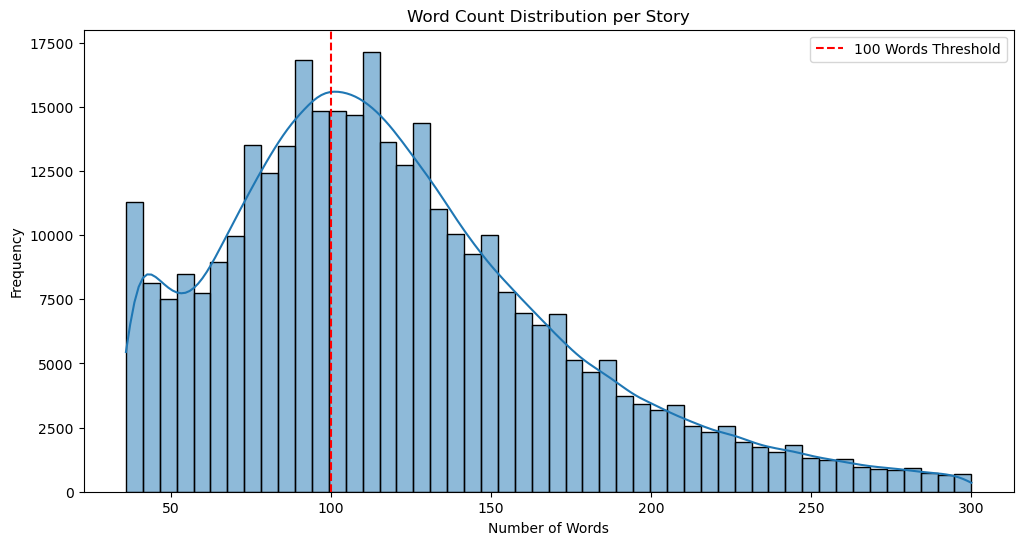
\includegraphics[width=.8\linewidth]{./images/histogramOriginalDataset.png}
    \caption{Original Dataset Histogram}
    \label{fig:histogram-original-dataset}
  \end{subfigure}
  
  \vspace{0.5cm} % Add some vertical space between the subfigures
  
  \begin{subfigure}[b]{\linewidth}
    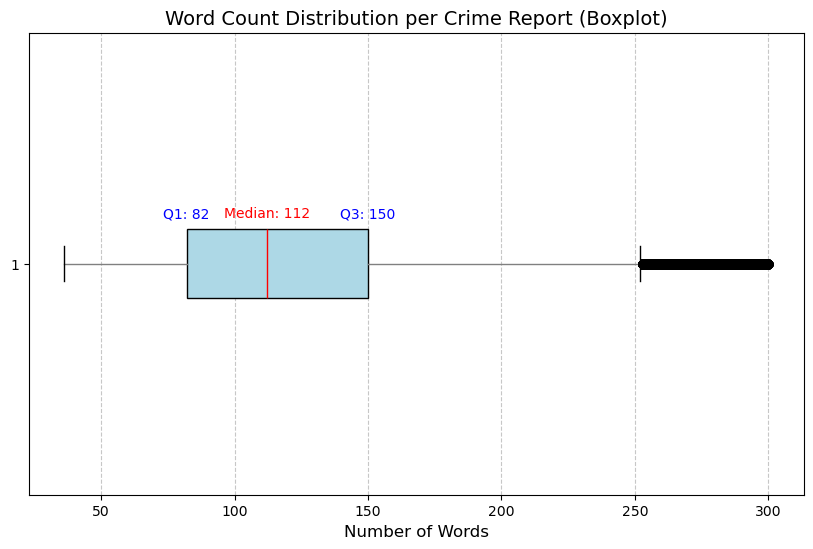
\includegraphics[width=.8\linewidth]{./images/boxPlotOriginalDataset.png}
    \caption{Box plot of Words Length in Original Dataset}
    \label{fig:boxplot-original}
  \end{subfigure}
  
  \caption{Distribution of word counts in collected data visualized through (a) a histogram  and (b)  a box plot}
  \label{fig:dataset-visualizations}
\end{figure}


% Meta-Llama-3-8B-Instruct
\subsubsection{Generative Artificial Intelligence Prompt Engineering}
\label{sec:prompt-engin-gai}


For this research, we used
Meta-\textsc{Llama}-3-8B-Instruct\cite{llama3modelcard}, an
instruction-tuned variant of Meta’s \textsc{Llama}~3 8B parameter
language model, optimized for conversational and task-oriented
interactions with multilingual capabilities. Built on a decoder-only
\textsc{Transformer} architecture, it leverages supervised fine-tuning
(\textsc{SFT}) and reinforcement learning from human feedback
(\textsc{RLHF}) to align responses with user intent. The model is
pre-trained on a diverse corpus of publicly available text data, with
enhancements in reasoning, coding, and safety mitigation compared to
its predecessors.

Prompt engineering is the process of crafting a suitable prompt to
drive the LLMs to solve a complex task, using natural language text
\cite{Zhao2023}. In this work, the LLM functions as an expert data
science assistant with the goal of constructing a dataset in the SQuAD
format in Spanish. For this purpose, the prompt receives the content
of the crime report as the \texttt{context} and each of the questions
from Table \ref{tab:commonquestions} as the \texttt{question}. The LLM
was also instructed to retrieve a \texttt{json} format output with the
variables: \texttt{context}, \texttt{question}, \texttt{answer\_text},
\texttt{answer\_start}, \texttt{answer\_end}, and
\texttt{impossible\_find\_answer}. The latter was calculated by
finding the \texttt{answer\_text} in the context. In the case that no
answer was possible to be retrieved, either because there is no answer
or because the LLM failed, the variable
\texttt{impossible\_find\_answer} was set to True.

\begin{table}[h]
\centering
\caption{Proposed Questions for the Dataset}
\label{tab:commonquestions}
\begin{tabular}{|p{0.9\textwidth}|}
\hline
\textbf{Question} \\
\hline
What objects were stolen? \\
% \hline
On what date did the incident occur? \\
% \hline
At what time did the robbery happen? \\
% \hline
At what address or between which streets did the robbery/incident occur? \\
% \hline
What was the dollar value of the stolen or taken objects? \\
\hline
\end{tabular}
\end{table}

Hugging Face's Inference API processed samples at a speed of 6.4
samples per minute. A total of 1,544 samples were obtained after four
hours. Our evaluation revealed two key limitations of the LLM: (1)
incomplete retrieval of answers for certain queries, and (2) sporadic
generation of irrelevant content. These results suggest that manual
verification of the generated dataset can aid in improving
quality. However, the engineered prompt allowed for the identification
of problems in generated samples.
\subsubsection{Dataset Quality}
\label{sec:dataset-quality}
After obtaining the initial \numprint{1544} samples (yielding \numprint{7705} total samples
when accounting for the five questions per context), we performed
quality assessment using the \texttt{impossible\_find\_answer} flag,
which identified approximately \numprint{3000} failure cases. We retained only
samples with \texttt{impossible\_find\_answer=False} and analyzed
answer lengths through histogram and box plot visualizations. This
revealed two key patterns: answers should be at most 17 words to be
considered valid, as we observed cases with zero-word
responses. A final curated dataset of \numprint{4572} samples for model training
and evaluation was obtained by selecting samples with a number of
words greater than 0 and where \texttt{impossible\_find\_answer=False}.


\subsubsection{Dataset Train and Test Split}
\label{sec:dataset-split}
The dataset was partitioned into training and testing sets, with 20\%
of the samples allocated for evaluation. The remaining 80\% were used
for training. This approach is a fundamental machine learning
technique that helps to evaluate the model's performance and
generalization capability. Table~\ref{tab:org63e879b} summarizes the
sample sizes for each subset. The split was performed randomly.

\begin{table}[htbp]
\caption{\label{tab:org63e879b}Dataset Train and Test Split}
\centering
\begin{tabular}{lr}
  \hline
Partition & \# Samples\\[0pt]
\hline
Train & \numprint{3657}\\[0pt]
  Test & \numprint{915}\\[0pt]
  \hline
  Total & \numprint{4572}\\[0pt]
  \hline
\end{tabular}
\end{table}
% check from here

\subsection{Model Fine-Tuning}
\label{sec:model-fine-tuning}
The
\texttt{mrm8488/bert-base-spanish-wwm-cased-finetuned-spa-squad2-es}
model was selected for fine-tuning because it is a model trained for
Spanish and QA tasks. As a matter of fact, it was tested without
training and it performed with an F1-Score of 81.70.

To fine-tune the model, both the question and the answer need to be
tokenized. As a result of this process, the indices indicating the
start and end of the answer must be recalculated based on the
tokenized embedding. In the case of long text, truncation should be
applied only to the context, and a window of 128 tokens was used to
avoid losing the answer during truncation. However, in this scenario,
since most of the current samples have no more than 100 words in the
context, this issue is unlikely to occur; nonetheless, it has been
addressed in the program.

In order to train the model, the parameters shown in Table
\ref{tab:org68816bf} were used. A small learning rate is recommended
for fine-tuning in order to reuse the pre-training from the original model and
adapt the new model to the target dataset. Our results prove that it
is possible to achieve a better performance on the target domain with
the fine-tuned model rather than using the pre-trained model. Although
the difference in performance is small, it could be related to the
fact that we were not able to use the whole dataset.

\begin{table}[htbp]
\caption{\label{tab:org68816bf}Training Parameters}
\centering
\begin{tabular}{ll}
  \hline
Parameter & Value\\[0pt]
\hline
Strategy & epoch\\[0pt]
Learning rate & \(2 \times 10^{-5}\)\\[0pt]
Batch Size & 64\\[0pt]
Epochs & 10\\[0pt]
Weight Decay & 0.01\\[0pt]
FP16 & True\\[0pt]
  Metric for best model & F1 (eval)\\[0pt]
  \hline
\end{tabular}
\end{table}
\section{Results}
\label{sec:results}

In this section, we present the results of fine-tuning the model,
along with the performance of the pre-trained model on the test
set. This comparison was conducted to determine whether the fine-tuned
model demonstrated any improvements over the original pre-trained
model. Table \ref{tab:before-performance} shows the performance of the
pre-trained model, while Table \ref{tab:finetunedModel} shows the
performance of the fine-tuned model. It is worth noting that the
latter improves upon the former. The fine-tuned model achieved an F1
score of 82.88 on the evaluation dataset. In this case, we use
\texttt{squad\_{v2}} which contains both the F1-SCORE and EXACT MATCH. A
function was prepared in order to be used by the Trainer Class.
\begin{table}
  \centering
  \caption{Pre-trained Model Performance}
  \label{tab:before-performance}
  \scriptsize
  \begin{tabular}{lr}
\toprule
Metric & Value \\
\midrule
eval\_loss & 0.9102 \\
eval\_model\_preparation\_time & 0.0077 \\
eval\_exact & 53.5519 \\
eval\_f1 & 81.7041 \\
eval\_total & 915.0000 \\
eval\_HasAns\_exact & 53.5519 \\
eval\_HasAns\_f1 & 81.7041 \\
eval\_HasAns\_total & 915.0000 \\
eval\_best\_exact & 53.5519 \\
eval\_best\_exact\_thresh & 0.0000 \\
eval\_best\_f1 & 81.7041 \\
eval\_best\_f1\_thresh & 0.0000 \\
eval\_runtime & 12.3982 \\
eval\_samples\_per\_second & 73.8010 \\
eval\_steps\_per\_second & 1.2100 \\
\bottomrule
\end{tabular}

\end{table}

\begin{table}
  \centering
  \caption{Fine-Tuned Model Performance}
  \label{tab:finetunedModel}
  \scriptsize
  \begin{tabular}{lr}
\toprule
Metric & Value \\
\midrule
eval\_loss & 1.0088 \\
eval\_model\_preparation\_time & 0.0077 \\
eval\_exact & 55.7377 \\
eval\_f1 & 82.8805 \\
eval\_total & 915.0000 \\
eval\_HasAns\_exact & 55.7377 \\
eval\_HasAns\_f1 & 82.8805 \\
eval\_HasAns\_total & 915.0000 \\
eval\_best\_exact & 55.7377 \\
eval\_best\_exact\_thresh & 0.0000 \\
eval\_best\_f1 & 82.8805 \\
eval\_best\_f1\_thresh & 0.0000 \\
eval\_runtime & 12.8109 \\
eval\_samples\_per\_second & 71.4240 \\
eval\_steps\_per\_second & 1.1710 \\
epoch & 10.0000 \\
\bottomrule
\end{tabular}

\end{table}



\section{Conclusions and Future Works}
\label{sec:conclusions}
In this study, we demonstrated the effectiveness of transformer-based
models for EQA within the context of criminal report analysis. Our
fine-tuned model showed a notable improvement, achieving an F1 score
of 82.88 compared to the pre-trained model's score of 81.70. This
indicates the potential for enhanced performance through
domain-specific fine-tuning.

The application of our model to robbery crime reports could facilitate
the extraction of crucial information, supporting legal practitioners
in their investigations and reporting. However, the study also
highlighted some limitations, including the model's occasional
inability to retrieve accurate answers and the need for manual
verification of results. 

Future work will aim to address these limitations by exploring
additional advanced techniques and incorporating manual labeling of
the dataset by expert peers. Additional computational resources will
also be required to process larger datasets. Furthermore, the
integration of AI into the legal domain holds significant promise for
more efficient case management and resource allocation, ultimately
contributing to a safer community. It is also of interest to
investigate other NLP techniques within the Ecuadorian legal context,
such as Legal Named Entity Recognition (NER) and Legal Document
Summarization (LDS). We encourage further research and collaboration
to refine these approaches and harness the full potential of AI in
supporting the justice system.



\begin{credits}
\subsubsection{\ackname} The authors would like to thank the Fiscalía
General del Estado for their cooperation in the development
of this research.

\subsubsection{\discintname}
The authors have no competing interests to declare that are relevant
to the content of this article.
\end{credits}
%
% ---- Bibliography ----
%
% BibTeX users should specify bibliography style 'splncs04'.
% References will then be sorted and formatted in the correct style.
%
\bibliographystyle{splncs04}
\bibliography{bibliography}
%
% \begin{thebibliography}{8}
% \bibitem{ref_article1}
% Author, F.: Article title. Journal \textbf{2}(5), 99--110 (2016)

% \bibitem{ref_lncs1}
% Author, F., Author, S.: Title of a proceedings paper. In: Editor,
% F., Editor, S. (eds.) CONFERENCE 2016, LNCS, vol. 9999, pp. 1--13.
% Springer, Heidelberg (2016). \doi{10.10007/1234567890}

% \bibitem{ref_book1}
% Author, F., Author, S., Author, T.: Book title. 2nd edn. Publisher,
% Location (1999)

% \bibitem{ref_proc1}
% Author, A.-B.: Contribution title. In: 9th International Proceedings
% on Proceedings, pp. 1--2. Publisher, Location (2010)

% \bibitem{ref_url1}
% LNCS Homepage, \url{http://www.springer.com/lncs}, last accessed 2023/10/25
% \end{thebibliography}
\end{document}

%%% Local Variables:
%%% mode: LaTeX
%%% TeX-master: t
%%% End:
